\documentclass[UKenglish]{beamer}


\usetheme{MathDept}
\usepackage{presentation}


%\setbeamerfont{title}{size = \fontsize{12.987}{14pt}} % Title on one line


\day = 8
\month = 11
\year = 2017

\title[\hspace{-1.6em}Join of hexagons and \CY threefolds]{Join of hexagons and \texorpdfstring{\CY}{Calabi--Yau} threefolds}
\subtitle{Public defence}
\author{Fredrik Meyer}


\begin{document}

\section{Outline} % 3
\begin{frame}
\frametitle{Outline of the thesis}

\begin{itemize}
	\item Unsuccessful attempt to find new hyper-Kähler varieties.
	\item The topology of $C(\dP6)$.
	\item New Calabi--Yau varieties and potential mirror partners.
\end{itemize}

\end{frame}

\section{Stanley--Reisner schemes} % 5
\begin{frame}
\frametitle{Stanley--Reisner schemes}


\begin{itemize}
    \item
    Given a simplicial complex $\mathcal F$, we get a Stanley--Reisner scheme $\P(\mathcal F)$.

    \item
    Is a union of projective spaces $\P^{\dim f}$, where $f$ is a face of $\mathcal F$.
\end{itemize}


\begin{example}

From a simplicial complex to a union of $\P^1$'s. \alert{Is the figure supposed to be asymmetric?}

\begin{center}
\tikzstyle{ball} = [circle,shading=ball, ball color=uiored,
    minimum size=0.01cm]
\begin{tikzpicture}
\coordinate (A) at (2.5,-1.2);
\coordinate (B) at (4.1, -1.2);
\coordinate (C) at (5, 0);
\coordinate (D) at (4.1, 1.2);
\coordinate (E) at (2.5, 1.2);
\coordinate (F) at (1.4, 0);

\draw[fill=red, fill opacity=0.4] (A) -- (B) -- (C) -- (D) -- (E) -- (F) -- cycle;

\node[style=ball, scale=0.5] at (A) {};
\node[style=ball, scale=0.5] at (B) {};
\node[style=ball, scale=0.5] at (C) {};
\node[style=ball, scale=0.5] at (D) {};
\node[style=ball, scale=0.5] at (E) {};
\node[style=ball, scale=0.5] at (F) {};

\draw (6.8,-1) -- (9.2,-1); % E_1
\draw (8.4,-1.2) -- (9.7,0.3); % L_12
\draw (7.6,-1.2) -- (6.3,0.3); % L_13
\draw (8.4,1.2) -- (9.7,-0.3);
\draw (7.6,1.2) -- (6.3,-0.3);
\draw (6.8,1) -- (9.2, 1); % L_23
\end{tikzpicture}
\end{center}

The ideal is generated by $x_ix_{i+2}=x_ix_{i+3}=0$ ($i=0,\ldots,5$).

\end{example}
\end{frame}


\begin{frame}
\frametitle{Stanley--Reisner schemes}

\begin{itemize}
	\item
	\alert{Join} of two subschemes $X$ and $Y$: The (closure of) the union of all lines between $X$ and $Y$.

	\item
	\alert{Join} of two Stanley--Reisner schemes $\P(\mathcal F)$ and $\P(\mathcal G)$ is $\P(\mathcal F \ast \mathcal G)$, where the faces of $\mathcal F  \ast \mathcal G$ are $f \sqcup g$ for $f \in \mathcal F$, $g \in \mathcal G$.
\end{itemize}

\pause

Smoothings of Stanley--Reisner schemes

\begin{itemize}
	\item Given a basis for $T^1(S_{\P(\mathcal K)},k)_0$, we can try to find a smoothing of $X_0 = \P(\mathcal K)$.
	\item A smoothing $X$ of $X_0$ will have many of the same properties:
		\begin{itemize}
			\item The same Hilbert polynomial.
			\item By semicontinuity, if $X_0$ is a sphere, $X$ will be \CY. %% which we define now
		\end{itemize}
\end{itemize}


\end{frame}

\section{Calabi--Yau varieties} % 5
\begin{frame}
\frametitle{\CY manifolds}

\begin{definition}%[\CY variety]
    A \alert{\CY variety} is a smooth projective scheme $X/\C$ of dimension~$3$ satisfying:
    \begin{itemize}
    	\item
	    $H^0(X,\OO_X)=H^3(X,\OO_X)=k$ and $h^1(X,\OO_X)=h^2(\OO_X)=0$.

	    \item
	    The canonical sheaf is trivial: $\omega_X \simeq \OO_X$. 
    \end{itemize}
\end{definition}

\unskip
\begin{columns}[onlytextwidth]
    \begin{column}{0.6\textwidth}
        \begin{itemize}
	        \item
	        Easiest invariants are the Euler characteristic and the Hodge numbers.

            \item
            We always have $\chi = 2(h^{11}-h^{12})$. 
        \end{itemize}
    \end{column}
\end{columns}

\only<1>
{
    \begin{textblock}{0.4}(0.58, 0.58)
        \[
            \arraycolsep = 1pt
            \def\arraystretch{0.5}
            \begin{array}[c]{ccccccc}
                &&& h^{00}                               \\  
                &&  h^{01} && h^{10}                     \\
                &   h^{02} && h^{11} && h^{20}           \\
                    h^{03} && h^{12} && h^{21} && h^{30} \\
                &   h^{13} && h^{22} && h^{31}           \\
                &&  h^{23} && h^{32}                     \\
                &&& h^{33} 
            \end{array}
        \]  
    \end{textblock}
}

\only<2>
{
    \begin{textblock}{0.4}(0.62, 0.62)
        \[
            \arraycolsep = 1.5pt
            \def\arraystretch{0.7}
            \begin{array}[c]{ccccccc}
                &&& 1                          \\
                &&  0 && 0                     \\
                &   0 && h^{11} && 0           \\
                    1 && h^{12} && h^{12} && 1 \\
                &   0 && h^{11} && 0           \\
                &&  0 && 0                     \\
                &&& 1 
            \end{array}
        \]
    \end{textblock}
}

\end{frame}
 
\section{Mirror symmetry} % 8
\begin{frame}
\frametitle{Mirror symmetry}

\begin{itemize}
	\item \CY threefolds seem to ``always'' have ``mirror partners''.
	\item Mirror partner $X^\circ$ to $X$ have ``mirrored Hodge diamond''.
	\item Hence $\chi(X^\circ) = - \chi(X)$.
\end{itemize}

\unskip
\begin{columns}[onlytextwidth]
    \only<1->
    {
        \begin{column}{0.48\textwidth}
            \[
                \begin{array}[c]{ccccccc}
                    &&& X                    \\
                    \hline                   \\[-1.8ex]
                    &&& 1                    \\
                    &&  0 && 0               \\
                    &   0 && 1   && 0        \\
                        1 && 101 && 101 && 1 \\
                    &   0 && 1   && 0        \\
                    &&  0 && 0               \\
                    &&& 1
                \end{array}
            \]
        \end{column}
    }

    \only<2->
    {
        \begin{column}{0.48\textwidth}
            \[
                \begin{array}[c]{ccccccc}
                    &&& \phantom{^\circ}X^\circ \\
                    \hline                      \\[-1.8ex]
                    &&& 1                       \\  
                    &&  0 && 0                  \\
                    &   0 && 101 && 0           \\
                        1 && 1   && 1 && 1      \\
                    &   0 && 101 && 0           \\
                    &&  0 && 0                  \\
                    &&& 1
                \end{array}
            \]
        \end{column}
    }
\end{columns}


\end{frame}

\section{Construction of new Calabi--Yau's} % 13
\begin{frame}
\frametitle{The cone over $\dP6$}

\begin{columns}
\column{0.5\textwidth}

\begin{itemize}
	\item Let $\dP6 \subset \P^6$ be an anticanonically embedded del Pezzo surface of degree $6$. Let $C(\dP6)$ be its affine cone in $\mathbb A^7$.

	\item The equations are 
	$$
\begin{vmatrix}
y & x_1 & x_2 \\
x_4 & y & x_3 \\
x_ 5 & x_6 & y
\end{vmatrix}
\leq 1
	$$

The origin is an isolated singularity.

\end{itemize}


\column{0.5\textwidth}

\begin{itemize}
	\item There are two smoothing components.
	\item They come from perturbations of differents form of writing the equation.
	\item Can also write the equations as:

	\begin{center}
	
	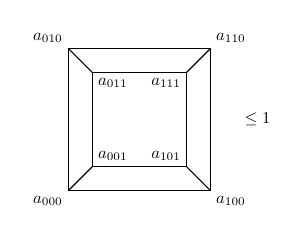
\begin{tikzpicture}[scale=0.6, every node/.style={scale=0.6}]
\draw (0,0) -- (3,0) -- (3,3) -- (0,3) -- cycle;
\draw (0.5,0.5) -- (2.5,0.5) -- (2.5,2.5) -- (0.5,2.5) -- cycle;
\draw (0,0) -- (0.5,0.5);
\draw (3,0) -- (2.5,0.5);
\draw (3,3) -- (2.5,2.5);
\draw (0,3) -- (0.5,2.5);
\node[below left] at (0,0) {$a_{000}$};
\node[below right] at (3,0) {$a_{100}$};
\node[above right] at (3,3) {$a_{110}$};
\node[above left] at (0,3) {$a_{010}$};

\node[above right] at (0.5,0.5) {$a_{001}$};
\node[above left] at (2.5,0.5) {$a_{101}$};
\node[below left] at (2.5,2.5) {$a_{111}$};
\node[below right] at (0.5,2.5) {$a_{011}$};

\node at (4, 1.5) {$\leq 1$};
\end{tikzpicture}
\end{center}
\end{itemize}


\end{columns}
\end{frame}
\begin{frame}
    \frametitle{Construction of a new \CY: $X_1$}

    \begin{itemize}
	    \item
        Let $E$ be a vector space with basis $e_1$, $e_2$, $e_3$. Consider
        \[
            \P^{17} = \P(E \otimes E \oplus E \otimes E).
        \]
        The elements are pairs of $3 \times 3$ matrices, equal up to scalar multiplication.

        \item
        Consider the set of pairs $M$ of matrices $(A, B)$ with rank $1 + 1$.

        \item
        Intersect $M$ with a generic $\P^{11} \subset \P^{17}\mkern-4mu$. Let $X_1 \defeq M \cap \P^{11}\mkern-4mu$.
    \end{itemize}

    \begin{theorem}
        $X_1$ is a smooth \CY with Euler characteristic $-72$.
    \end{theorem}
\end{frame}


\begin{frame}
    \frametitle{Construction of a new \CY: $X_2$}

    \begin{itemize}
    	\item Let $F$ be a vector space with basis $f_1$, $f_2$. Consider
	    \[
            \P^{15} = \P(F \otimes F \otimes F \oplus F \otimes F \otimes\alert{????}).
	    \]
	    The elements are pairs of $2 \times 2 \times 2$-tensors, equal up to scalar multiplication.

	    \item
	    Consider the set of pairs $N$ of tensors $(A, B)$ with rank $1 + 1$.

	    \item
	    Intersect $N$ with a generic $\P^{11} \subset \P^{15}\mkern-4mu$. Let $X_2 \defeq N \cap \P^{11}\mkern-4mu$.
    \end{itemize}

    \begin{theorem}
        $X_2$ is a smooth \CY with Euler characteristic $-48$.
    \end{theorem}
\end{frame}

\begin{frame}
    \frametitle{Construction of a new \CY: $X_3$}

    \begin{itemize}
    	\item
    	Let $E$ and $F$ be as before. Consider
        \[
            \P^{16} = \P(E \otimes E \oplus F \otimes F \otimes\alert{????}).
        \]
        
        \item
        Consider the set of pairs $W$ of tensors $(A, B)$ with rank $1 + 1$.

        \item
        Intersect $W$ with a generic $\P^{11} \subset \P^{16}\mkern-4mu$. Let $X_3 \defeq  W \cap \P^{11}\mkern-4mu$.
    \end{itemize}

    \begin{theorem}
        $X_3$ is a smooth \CY with Euler characteristic $-60$.
    \end{theorem}
\end{frame}

\begin{frame}
    \frametitle{Hodge number heuristics}

    \begin{conjecture}
        $X_1$ has Hodge numbers $h^{11}\mkern-3mu = 3$ and $h^{12}\mkern-2mu = 39$.
    \end{conjecture}

    \begin{proof}[``Reason'']
        \begin{enumerate}[<+->]
            \item
	        We know the Euler characteristic, so it is enough to find $h^{12}$ ($=$ number of parameters).

            \item
            The Grassmannian of $\P^{11}$'s in $\P^{17}$ is $72$-dimensional.

            \item
            We can act by automorphism from $\prod_{i = 1}^4 \GL(E)$.

            \item
            The subgroup $\{ t_1t_2 = t_3t_4 \} \subset (\C^\ast)^4 \subset \prod_{i = 1}^4 \GL(E)$ acts trivially.
            \vspace*{-0.5ex}

            \item
            Hence $h^{12} = 72 - \Big(\dim \prod_{i = 1}^4 \GL(E) - 3\Big) = 72-33 = 39$.
            \qedhere
        \end{enumerate}
    \end{proof}
\end{frame}
\begin{frame}
\frametitle{Mirror candidate for $X_1$}

Using the mirror Ansatz, we propose mirror candidates for $X_1$ and $X_2$.

\begin{itemize}[<+->]
	\item
	There is an $H \defeq \Z/3$-action on $E$ defined by $e_i \mapsto \omega^i e_i$.

	\item
	Another $\Z/3$-action $e_i \mapsto e_{i + 1}$.

	\item
	Extend to actions on $\P\big((E \otimes E) \oplus (E \otimes E)\big) = \P^{17}\mkern-4mu$.

	\item
	Choose invariant $\P^{11}$: Defined by
	\[
	    f_{ij}^\alpha = e_{ij}^\alpha + t_{-i-j}^\alpha e_{-i-j,-i-j}^{\alpha+1}
	\]
	for $i,j \in \Z/3 \times \Z/3$ ($i \neq j$) and $\alpha = 0,1$.

	\item
	The resulting $X_{H_t} \defeq \P^{11} \cap M$ is singular with $48$ isolated double point singularities.
\end{itemize}

\end{frame}

\begin{frame}
\frametitle{Mirror candidate for $X_1$}

\begin{itemize}
	\item We divide out by the $H$-action and resolve: $X_1^\circ \defeq \widetilde{X_{H_t}/H}$.
	\pause
	\item Roan's formula gives:
	\[
	    \chi(X_1^\circ) = \frac{1}{3} \left(24 + 8 \cdot 24\right) = 72.
	\]
\end{itemize}

Based on this calculation and the mirror heuristic, we conjecture:

\begin{conjecture}
    $X_1^\circ$ is a mirror of $X_1$.
\end{conjecture}

\pause
\begin{remark}
    A very similar construction gives a mirror candidate for $X_2$.
\end{remark}

\end{frame}


\end{document}